\chapter{Harmonogram realizacji projektu}
\label{ch:harmonogram}

\section{Główne etapy tworzenia aplikacji}
Poniżej wypisano główne fazy prac i implementacji w kolejności ich faktycznej realizacji:

\begin{enumerate}
    \item \textbf{Przygotowanie bazy danych} -- Zaprojektowanie schematu relacyjnej bazy danych na podstawie opracowanego wcześniej diagramu ERD.
    \item \textbf{Budowa podstawy aplikacji} -- Stworzenie podstawowych okien interfejsu użytkownika, w tym \texttt{LoginWindow} oraz \texttt{MainWindow}, definiujących szkielet aplikacji w WPF.
    \item \textbf{Przygotowanie podstawowych widoków} -- Zaimplementowanie paneli Powiadomień, Wydarzeń, Ofert oraz Transakcji, wraz z obsługą powiązanej z nimi logiki biznesowej.
    \item \textbf{Moduł klientów i autoryzacji personelu} -- Stworzenie widoku zarządzania użytkownikami, obejmującego pełną obsługę operacji CRUD dla rekordów z bazy danych.
    \item \textbf{Stworzenie modułu kodów QR} -- Przygotowanie metod odpowiedzialnych za sprawne generowanie, jak również skanowanie i weryfikację kodów QR z poziomu okna aplikacji.
    \item \textbf{Panel menadżera} -- Dodanie i konfiguracja zbiorczego widoku podsumowania (wyświetlającego najważniejsze statystyki utargów i wejść), dedykowanego wyłącznie dla menedżerów.
    \item \textbf{Algorytmy biometryczne} -- Zaprojektowanie i wdrożenie algorytmu hashowania odcisków palców.
    \item \textbf{Narzędzia pobierania danych biometrycznych} -- Przygotowanie wbudowanego mechanizmu do pobierania próbek i przypisywania cyfrowych wzorców odcisków do konkretnego klienta w bazie.
    \item \textbf{Symulator skanera biometrycznego} -- Stworzenie okna symulującego proces skanowania odcisków palców oraz autoryzacji klienta.
    \item \textbf{Pisanie dokumentacji} -- Proces ciągły, realizowany od momentu przygotowania bazy danych, aż po aktualne wprowadzane zmiany.
    \item \textbf{Finalne łatki i poprawki} -- Ostatnie szlify i korekty w kodzie, obejmujące komentowanie kodu i debugowanie.
\end{enumerate}

\section{Wizualizacja harmonogramu}
Dla lepszego zobrazowania rozkładu prac w czasie i zależności między poszczególnymi zadaniami, przygotowano wykres harmonogramu obrazujący omówione wyżej punkty. Zaznaczono w nim między innymi fakt ciągłości prac nad dokumentacją w relacji z kodowaniem oprogramowania.

\begin{figure}[H]
    \centering
    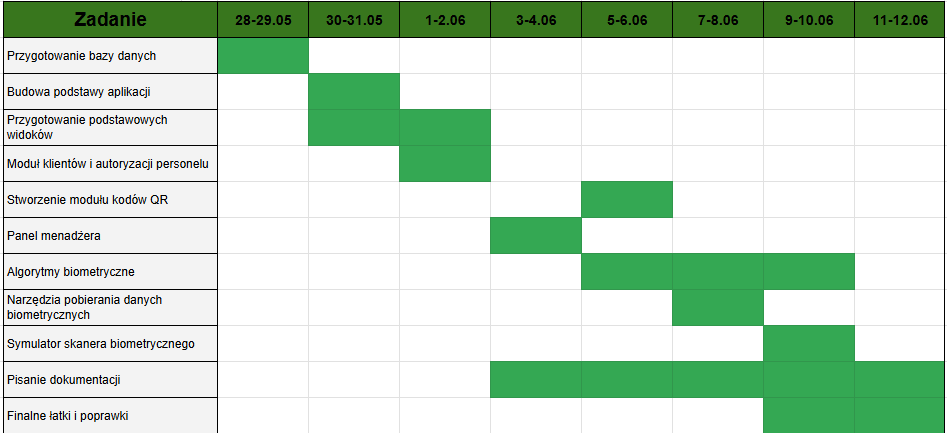
\includegraphics[width=0.9\textwidth]{figures/diagramGantta.png}
    \caption{Diagram przedstawiający harmonogram prac projektowych}
    \label{fig:harmonogram_gantt}
\end{figure}
